\documentclass[a4paper,11pt,oneside, titlepage]{article}
\usepackage[a4paper]{geometry} 
\geometry{a4paper,left=25mm, right=25mm, top=20mm, bottom=30mm} 
\usepackage[ngerman]{babel}
\usepackage[utf8x]{inputenc}
\usepackage[T1]{fontenc}
\usepackage{fancyhdr}
\usepackage{hyperref}
\usepackage[table]{xcolor}
\renewcommand{\arraystretch}{2}
\renewcommand\thesubsection{}

\pagestyle{fancy}

\lhead{\today}
\rhead{Verantwortlicher: Franz Ruge }
\chead{Gruppe: na17b}
\title{Lastenheft\\Nachrichtenkommunikation für das THW}
\author{na17b}
\date{}

\begin{document}
\maketitle
\tableofcontents
\newpage


\section{Ausgangssituation}
Die Grundlage für dieses Projekt bildet der sogenannte Vierfachvordruck, ein 
internes Kommunikationsdokument des technischen Hilfswerks (THW). Es wird in 
der mobilen Einsatzzentrale des THW, der Fachgruppe Führung und Kommunikation 
(FGr FK) eingesetzt. Die FGr FK nutzt das Dokument, um ein- und ausgehende 
Nachrichten abzufassen und so z.B. Einsatzaufträge für Einheiten, eingehende 
Lagemeldungen oder Materialanforderungen abzuarbeiten. Der Vierfachvordruck 
ist eine Papier-Vorlage mit dreifachem Durchschlag. Zwei der Durchschläge 
werden an die zuständigen Personen innerhalb der FGr FK verteilt. Der dritte 
Durchschlag dient der Protokollierung. Im Angesicht heutiger Technologien 
erscheint dieses Verfahren nicht mehr zeitgemäß. Mithilfe einer Software wäre 
es möglich, den Prozess digital durchzuführen. Dadurch müssten keine 
handschriftlichen Dokumente verfasst und verteilt werden und das Verfahren 
könnte beschleunigt werden. Alle Nachrichten und Nachrichtenverläufe ließen 
sich leicht in einer Datenbank archivieren. Ein weiterer Vorteil wäre der 
Entfall von Mehraufwand durch schlecht lesbare Handschrift. Außerdem ließe 
sich die Verwaltung verschiedener Dokumente am Arbeitsplatz übersichtlicher 
gestalten, etwa durch ein digitales Postfach.

\section{Zielsetzung und Produkteinsatz}
Ziel des Projekts ist es, eine Anwendung zu schreiben, welche es erlaubt, einen Vierfach-Vordruck
abzufassen, anzuzeigen und zu archivieren sowie den damit verbundenen Workflow zu durchlaufen, 
welcher lediglich durch die Software ergänzt aber nicht ersetzt werden soll. 
Zur maximalen Kompatibilität soll es sich um eine Browseranwendung handeln, welche ihre Daten in
einer versionierten RDF-Datenbank auf Serverseite ablegt. 
Die Archivierung muss dabei die rechtliche Verbindlichkeit sicherstellen, d.h. nachträgliche
Änderungen an den Dokumenten sollen erkennbar sein und verhindert werden.
Die Software soll innerhalb der Fachgruppe Führung/Kommunikation eingesetzt werden um den Austausch 
von ein- und ausgehenden Nachrichten zu beschleunigen und zu vereinfachen.


\section{Nichtfunktionale Anforderungen}
\subsection{/LF0000/ Ähnlichkeit zum Papierformular}
Der simulierte Vierfachvordruck sollte in Form und Formulierung dem Papierformular gleichen. Somit soll der gewohnte Arbeitsablauf gewährleistet werden. 
\subsection{/LN0100/ Listenanordnung für Vierfachvordrucke}
In dem Fall, dass zeitgleich mehr als ein Vierfachvordruck bei einem Mitarbeiter ankommt, sollte eine Liste zum Abrufen der eingegangen Dokumente existieren. Somit kann jedes Dokument nacheinander bearbeitet werden, wodurch es auch zu keinem Informationsverlust kommen kann.
\subsection{/LF0400/ Archivierung}
Es ist von immenser Bedeutung für das Technische Hilfswerk, nach eininger Zeit wieder auf die Angaben eines Vierfachvordrucks
zugreifen zu können. Momentan wird dies ermöglicht, indem eine Kopie des Zettels im Archiv geordnet abgelegt wird. Da wir das manuelle Ausfüllen eines Vierfachvordrucks mit unserer Applikation abschaffen wollen, müssen wir dafür sorgen, dass die Archivierung trotzdem noch aktiv gehalten werden kann. Das heißt, es ist unbedingt erforderlich, dass die Eingaben, die digital getätigt werden, ausdruckbar sind. Dabei sollte die Darstellungsform der analogen Zettel möglichst beibehalten werden, um die Archivierung einheitlich zu halten. Und weil doppelt immer besser hält, sollen die Eingaben auch noch längerfristig auf einem Server gespeichert werden, um u.a. einen noch schnelleren Zugriff zu ermöglichen. Dieser Server ist derselbe wie der, über den unser Programm später laufen soll, ist somit also nur lokal zugreifbar.
\subsection{Kommunikation zwischen Computern}
Zur Weiterleitung des (ausgefüllten) Dokuments von Mitarbeiter zum Mitarbeiter müssen Computer untereinander kommunizieren können. Gegenüber äußeren unbefugten Zugriffen sollten die Computer sowie der Kommunikationsweg geschützt sein.
\subsection{verschiedenen Rollen}
Zum Zwecke der besseren Übersicht und Nachbildung des Workflows ist die Aufteilung in verschiedene Rollen sinnvoll.  
Dabei kann gewährleistet werden, dass jeder nur das sieht und machen kann, was für ihn relevant ist und so die Fehleranfälligkeit minimiert wird. 
Die Auswahl der jeweiligen Rolle erfolgt dabei vor jedem Einsatz über ein Menü. Somit ist nicht ein PC an eine Rolle gebunden und man kann sein Setup frei wählen, das heißt beliebig viele Rollen einer Art hinzufügen.

\subsection{/LN0000/ Skalierbarkeit}
Das System der Vierfachvordrucke bietet die Möglichkeit, dass auch mehrere Personen eine Rolle übernehmen, also dass es zum Beispiel zwei oder mehr Funker gibt. Dies ist notwendig, da unterschiedliche Notlagen unterschiedlich stark besetzte Teams erfordern um bewältigt zu werden. Demnach ist es wichtig, dass mit der Software umsetzbar ist, dass eine bestimmte Position zu unterstützenden Zwecken mehrfach besetzt werden kann. Daraus folgt, dass mindestens elf Personen gleichzeitig in der Applikation arbeiten können. Zu achten ist dabei vor allem auf Konflikte bei der gleichzeitigen Bearbeitung von Vordrucken.

\section{Funktionale Anforderungen}
\subsection{/LF0000/ Visuelle Unterschiede für verschiedene Rollen}
Die visuelle Representation orientiert sich an der Gestaltung des Vierfachvordrucks. Dabei wird vor Allem die Farbgebung weitergeführt,   
d.h. jede Ansicht wird thematisch in der Farbe des für sie relevanten Vordruckes gehalten. Jede Rolle bekommt ihre eigene Ansicht.  
Dies dient vor allem der Übersichtlichkeit und Einfachheit der benutzung, da jede Rolle somit nur das sieht, was sie auch wirklich brauch.  


\subsection{/LF0100/ Vierfachvordruck renderbar als PDF}
Um die manuelle Archivierung zu gewährleisten, sollten die digital getätigten Eingaben ausdruckbar sein. Dabei sollte möglichst Einheitlichkeit beibehalten werden, d.h. alle Eingaben müssen so in eine digitale Version des Vierfachvordrucks geschrieben werden, wie es der Verfasser auch tun würde. Die Vorlage sollte dabei möglichst in ein PDF konvertiert werden, um gutes Ausdrucken zu gewährleisten. Das Ausdrucken sollte auch so benutzerfreundlich wie möglich vonstatten gehen, also mit abgespeicherter, aber veränderbarer, Vorkonfiguration welche auf einen Knopfdruck abgeschickt werden kann.
\newpage
\subsection{/LF0200/ Speicherung im RDF-Format}
Die vom Verfasser im Vierfachvordruck eingegebenen Informationen, sollen im RDF Datenmodell mithilfe des im QuitStore verfügbaren SPARQL-Endpoints auf einem lokalen Server abgespeichert werden. Demnach werden die Eingaben, z.B. 'Dokument hat Absender: Nathanael Arndt' in folgender Form dargestellt:
\begin{flushleft}
\quad \quad \quad Subjekt Vierfachvordruck (repräsentiert durch URI) \\
\quad \quad \quad Prädikat `hatAbsender' \\
\quad \quad \quad Objekt `Natanael Arndt' (repräsentiert durch URI oder Name)
\end{flushleft}
Die anderen Stationen, die bisher Kopien des Vierfachvordrucks erhalten haben, müssen nun digital auf die Eintragungen des Verfassers zugreifen können. Dies wird direkt durch den SPARQL-Endpoint ermöglicht, welcher eine Oberfläche für gezielte SPARQL-Abfragen an das Datenmodell bietet.
\subsection{/LF0300/ Verschlüsselung}
Die Verschlüsselung sollte nach einem standartisierten oder offen und frei nachvollziebaren Verfahren ablaufen, damit juristische Integrität gewährleistet ist. 
Dieser Teil wird in diesem Fall von QuitStore übernommen, was durch die Überschneidung mit Git dessen Versionierung nutzt. Dadurch wird natürlich auch die cryptografische Eindeutigkeit gewährleistet, da die Git-History durch auf einander aufbauende Hash-Codes gesichert ist. Das heißt ändert man etwas an zum Beispiel einem Commit, werden auch alle IDs der Commits usw. danach geändert.

\subsection{/LF0600/ Datensicherheit}
Die Vordrucke werden nach ihrer Erstellung und Durchlaufens des weiteren Prozesses abgespeichert.
Damit eine Archivierung der Vordrucke sinnvoll ist, muss sichergestellt werden, dass sie von niemandem  
nachträglich verändert werden können. Ansonsten verliert das Archiv jegliche juristische Relevanz und das THW die Möglichkeit nachzuvollziehen wo und warum Fehler aufgetreten sind. Demnach muss die Eindeutigkeit der gespeicherten Daten gewährleistet sein. 

\subsection{Zugriffsbeschränkung der Nutzer}
Der Vierfachvordruck hat Abschnitte, die nur von speziellen Mitarbeitern ausgefüllt werden dürfen. Dies sollte auch in der Software beachtet werden. So soll jeder Mitarbeiter nur den zu ihn gehörenden Abschnitt bearbeiten beziehungsweise beschreiben, wodurch Verfälschungen des Dokuments verhindert werden sollen.

\section{Use-Cases}

\subsection{/LC0000/ Auswahl der Rolle}
Das System bietet dem Nutzer die möglichkeit eine der folgenden Rollen auszuwählen
\begin{itemize}
\item Sachbearbeiter (S1-S6)
\item Sichter
\item Leiter der Fernmeldezentrale (LDF)
\item Funker
\end{itemize}

\newpage
\subsection{/LC0100/ Ausgehende Nachrichten}
\begin{figure}[htpb]
	\centering
	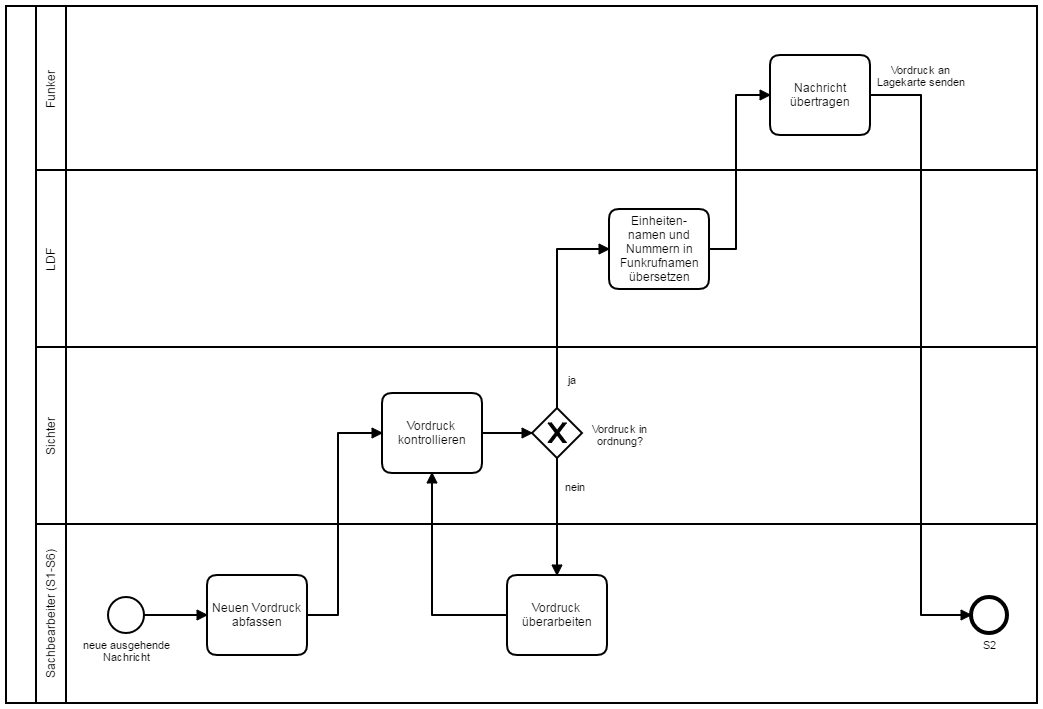
\includegraphics[width=0.95\linewidth]{ausgehend.png}
\end{figure} Ein Sachbearbeiter erhält eine neue ausgehende Nachricht und fasst einen neuen Vordruck ab. Dieser Vordruck wird von einem Sichter kontrolliert und an den LDF übermittelt. Der LDF übersetzt die Einheitennamen und Nummern in Funkrufnamen bevor der Vordruck an den Funker zur Übertragung weitergeleitet wird. Im Anschluss daran erhält Sachbearbeiter S2 (Lagekarte) den Vordruck, womit der Vorgang abgeschlossen wird.

\newpage
\subsection{/LC0200/ Eingehende Nachrichten} 
\begin{figure}[htpb]
	\centering
	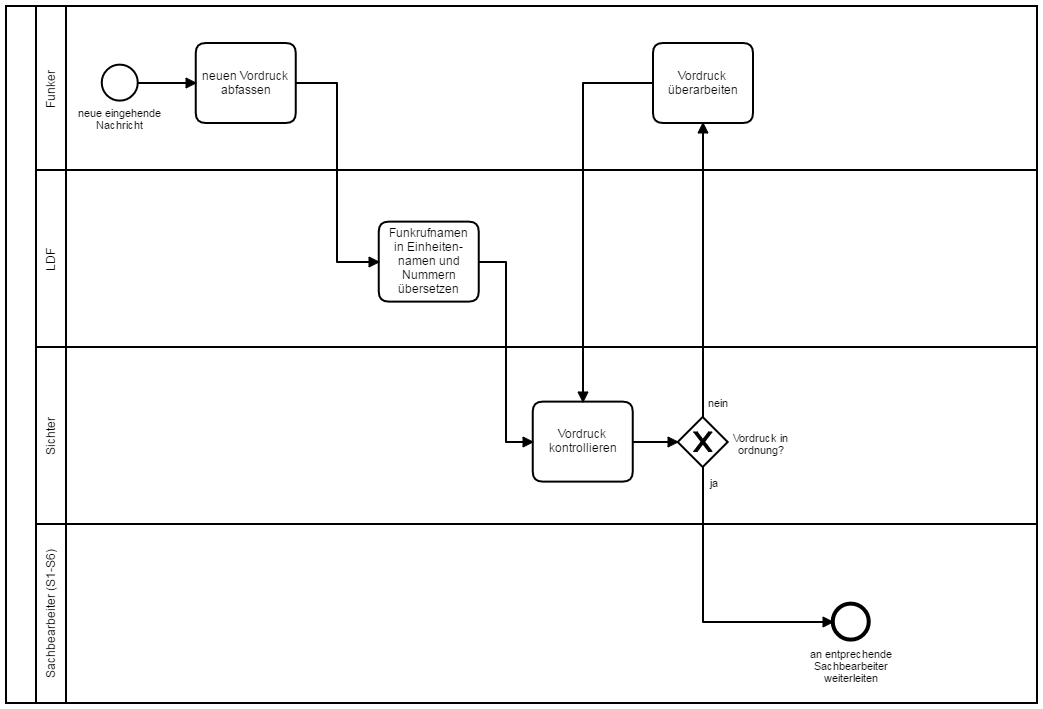
\includegraphics[width=0.95\linewidth]{eingehend.png}
\end{figure} Ein Funker erhält eine neue eingehende Nachricht und fasst einen neuen Vordruck ab. Der LDF übersetzt die Funkrufnamen in Einheitennamen und Nummern bevor der Vordruck zur Kontrolle an einen Sichter gesendet wird. Anschließend wird der Vordruck an die entprechenden Sachbearbeiter übermittelt

\subsection{/LC0300/ Kontrolle durch Sichter}
Ein Sichter erhält einen Vordruck zur Kontrolle und stuft diesen als unzureichend ein. Der Vordruck wird dann zurück an den Verfasser gesendet, welcher diesen überarbeitet und zur erneuten Kontrolle an den Sichter schickt. Wird ein Vordruck vom Sichter erfolgreich abgenommen durchläuft er den weiteren Workflow.

\subsection{/LC0400/ Ausdrucken eines Vordruckes}
Das System bietet dem Nutzer die Möglichkeit, sich einen verfassten oder erhaltenen Vordruck anzuschauen und auszudrucken.

\section{Qualitaetsmatrix}

    \begin{tabular}{ |l|l| }
        \hline
        \multicolumn{2}{ |c| }{Qualitaetsmatrix nach ISO 25010} \\
        \hline
        Qualitätskriterium & Gewichtung  \\ \hline
        Zuverlässigkeit (Reliability) & Hoch\\ 
        Gebrauchstauglichkeit (Usability) & Hoch\\ 
        Funktionalität (Functional Suitability) & Mittel\\ 
        (IT-)Sicherheit (Security) & Mittel\\ 
        Wartbarkeit (Maintainability) & Mittel\\ 
        Effizienz (Performance Efficiency) & Niedrig\\ 
        Portabilität (Portability) & Niedrig\\ 
        Kompatibilität (Compatibility) & Niedrig\\ \hline
        \end{tabular}
    

\section{Lieferumfang und Abnahmekriterien}
Das fertige Produkt umfasst eine voll funktionale Webseite, welche innerhalb einer mobilen Einsatzzentrale die Arbeit mit dem Vierfachvordruck vollkommen ersetzen kann. Aufgrund der großen Verantwortung des THW ist die Zuverlässigkeit der Software besonders wichtig. Um diese zu gewährleisten muss die Software und deren Module vor ihrer Auslieferung und während der Entwicklung vollumfänglichen automatisierten Tests unterzogen werden. Wofür ein noch zu wählendes Testingframework Anwendung findet, welches vorrausichtlich der Unit-Reihe entstammen wird. Eine weitere Komponente ist das zuverlässige Speichern, Abfragen und Darstellen der ausgefüllten Vordrucke. Hierzu wird ein Datenbanksystem aufgesetzt, welches das RDF-Modell verwendet, SPARQL als Querylanguage unterstützt und die Quit-Store Speicher-Architektur nutzt. Die Darstellung orientiert sich stark am Original des Vierfachvordrucks und erfolgt über eine Webseite. Um die Verlässlichkeit weiter zu steigern wird darüber hinaus das Prinzip der kontinuierlichen Integration angewandt. Somit kann eine gemeinsame, einfach erreichbare und verlässliche Codebasis für das gesamte Team geschaffen werden. Ein weiteres wichtiges Abnahmekriterium ist die hohe Gebrauchstauglichkeit, welche eine wichtige Vorraussetzung für die Akzeptanz der Software ist. Hierbei ist insbesondere die schnelle Zugänglichkeit, die klare Trennung der Rollen und die Möglichkeit des Effizienten und schnellen Arbeitens zu gewährleisten. Aus der geforderten Usability folgt auch eine entsprechende Performanz, welche das unterbrechungsfreie, parallele Arbeiten von bis zu acht Nutzern (vier Sachgebietsbearbeiter, zwei Funker, ein Sichter und ein Stabsleiter) garantiert, wobei als Hardware ein Raspberry Pi vorgesehen ist. Um die Akzeptanz weiter zu steigern, soll die Software in der Lage sein den Nutzern durch ihre Funktionalität weitere Aufgaben abzunehmen oder zumindest zu erleichtern. Dazu seien bspw. das Drucken der rechtlich belastbaren Unterlagen und die verschiedenen Sichten mit ihren Zugriffsbeschränkungen genannt. Im Hinblick auf die mögliche Weiterentwicklung ist auch die Wartbarkeit durch eine ausführliche, wohl strukturierte Dokumentation, sowie einheitlich formatierten und gut leserlichen Code möglichst komplikationsfrei zu gestalten. Die Kompatibilität muss in sofern gegeben sein, dass die Webseite auf unterschiedlichen Geräten gut erkenn- und bedienbar sein soll. Durch die feste Hardware ist die Portabilität weniger wichtig, trotzdem sollte die Möglichkeit bestehen ohne großen Aufwand auf ein anderes System zu migrieren. 

\subsection{Vorprojekt}

    Der Fokus im Vorprojekt liegt auf der Erstellung der Benutzeroberfläche zur Erstellung eines Vierfachvordrucks. 
    Die GUI wird über den Browser aufgerufen und ermöglicht in der Startseite die Auswahl der entsprechenden Rolle über 
    ein Dropdown-Menü. In derselben Übersichtsseite sind die für die ausgewählte Rolle relevanten Informationen ersichtlich. 
    Jede Rolle hat einen eigenen View. Einen neuen Vordruck zu erstellen ist für jeden Nutzer möglich, dabei soll das 
    Design des Formulars im Vorprojekt weitestgehend fertig umgesetzt sein.
    
    Zu Demonstrationszwecken sollen einige fest voreingestellte Vordrucke zur Verfügung stehen. Neu erstellte Vordrucke
    bleiben zunächst nur temporär bestehen und gehen beim Verlassen der Seite verloren. Dadurch sollen Testnutzer
    in der Lage sein, einen ersten Überblick über den Prozess der Verfassens eines Vierfachvordrucks zu erhalten,
    ohne sich Gedanken über die Integrität der Daten machen zu müssen.

    Der Workflow liegt hierbei zunächst nicht im Fokus; dieser wird erst im fertigen Projekt ersichtlich sein, da hierzu
    ein funktionsfähiges Backend benötigt wird.


\newglossaryentry{Jest} {
  name=Jest,
  description={
    Von Facebook entwickeltes Testframework für Javascript. Zeichnet sich durch seine Einfachheit in der Benutzung aus.
  }
}
\newglossaryentry{vue-test-utils} {
  name=vue-test-utils,
  description={
    Sammlung an Funktionen um Vue-Komponenten in Unit-Tests verwenden zu können.
  }
}
\newglossaryentry{GitLab CI} {
	name=GitLab CI,
	description={
		GitLab CI ist die in GitLab eingebaute Continous Integration, die sich mit Hilfe der gitlab-ci.yml Datei konfigurieren lässt.
	}
}

\end{document}
